
%%% Local Variables: 
%%% mode: latex
%%% TeX-master: "main"
%%% End: 
\section{Resolving Misassembly}

These examples illustrated some common themes for misassemblies throughout the genome, notably the effect of background signal from high depth sequencing. Three types of misassemblies were described: extension, fusion, and truncation. In all cases these errors were resolved by solved by combining signals from sequencing depth and genome annotations. The assembly was fully curated for all pSol1 transcripts (the pSol1 megaplasmid is 5\% of the genome). This section explicitly states the rules and heuristics used for assembly curation. Also, the assembly was analyzed before and after curation to demonstrate the effectiveness of this technique. 

The curation process was used in the previous section to address the misassemblies, providing precision transcript boundary estimates. This technique used heuristic techniques to correct transcript boundaries according to reflect depth and annotations in cases where interfering signals result in misassembly. Background signals were defined as extended (typically intergenic or antisense) regions of low depth that frequently conflicted with matching promoter/terminator annotations and large depth fold changes of transcript termini. Briefly, the heuristics are as follows:

\begin{enumerate}
\item Weak terminators ($\delta$G \textgreater -6kcal/mol) were omitted from analysis.
\item Weak promoters and TFBSes were excluded from analysis when p \textgreater 1\e{-5}, defined below where p is defined below for upstream and downstream motif matches (e.g. -35 and -10 elements of $\sigma$_{A} promoter). 
\[ p_{promoter} = p_{upstream} \times p_{downstream} \]
\item Extended transcripts were corrected by shortening or spliting transcripts, such that the resulting transcript(s) captured depth patterns and annotations.
\item Fused transcripts were similarly addressed, although terminators were increasingly important in these cases.
\item Truncated transcripts typically accompanied obvious trends in depth (e.g. BdhA) and were corrected by extension of the transcript to termini suggested by both depth and genome annotation.
\item Almost always, two or more signals (i.e. depth, terminator, etc.) in agreement were used to determine the true transcript boundaries. In edge cases, extended location specific differences in depth (\textless 2 fold change) that were consistent across replicates were determined to be a transcript terminus.
\end{enumerate}

\begin{table}
\caption{Curation Effect}\label{table:assemb_curation}
\begin{center}
\begin{tabular}{|c|c|c|}\hline
  & Uncurated & Curated\\\hline\hline
Transcripts & 181 & 111\\\hline
Sequenced Mb & 347413 & 192069\\\hline
Length Range & 202-16389 & 172-11397\\\hline
CDSes & 155 & 157\\\hline
Standard Transcripts & 59 & 86\\\hline
Standard Mb & 246926 & 174801\\\hline
Novel Transcripts & 122 & 24\\\hline
Novel Mb & 100487 & 14994\\\hline
\end{tabular}
\end{center}
\end{table}

\begin{wrapfigure}{R}{0.4\textwidth}
\small
\vspace{-20pt}
\begin{center}
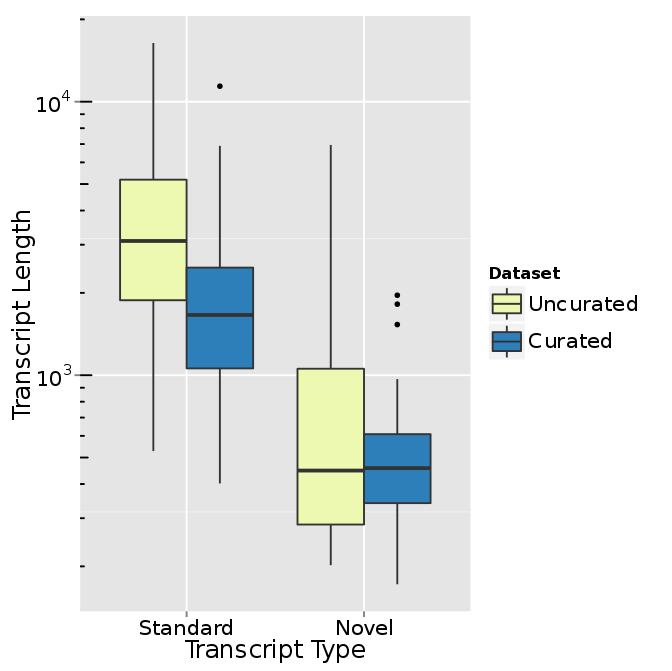
\includegraphics[width=\linewidth,height=3in]{images/Assembly/Curation/PairvsCuration_length.png}
\end{center}
\vspace{-20pt}
\caption{Transcript Lengths}\label{fig:5.20}
The transcript lengths were improved after curation, centering the distribution on the standard transcripts on the \textit{E. coli} average\cite{86}.
\end{wrapfigure}

These heuristics guided the curation process, addressing the errors described in previous sections, similarly to the treatment of the example transcripts. The most common types of misassemblies were the result of residual background signal assembled mixed with true genic signal. The three types of errors were corrected by curation of the entire pSol1 megaplasmid, resulting in 111 transcripts spanning 192kb (\ref{table:assemb_curation}). In addition to improving the precision of transcript boundary determination, the type I error for transcript discovery was reduced by removing a large number of false positive transcripts.

\begin{figure}
\begin{center}
\begin{minipage}{.48\textwidth}
\begin{center}
{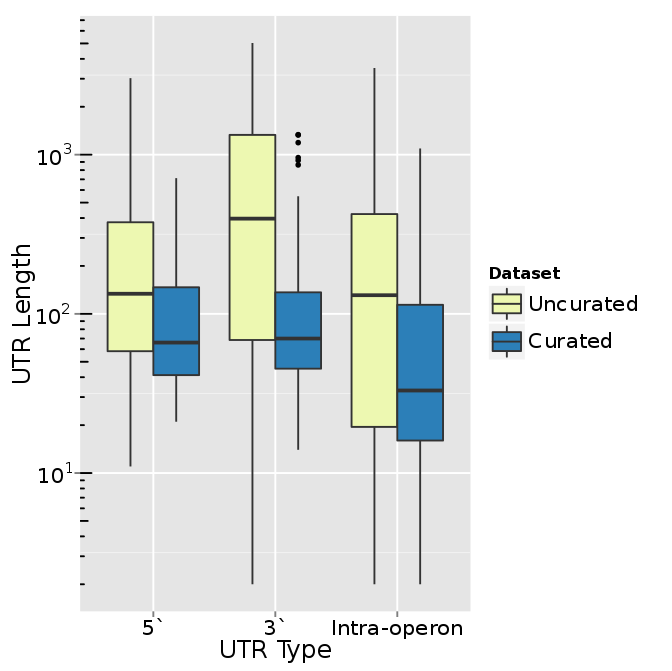
\includegraphics[width=\linewidth,height=3in]{images/Assembly/Curation/PairvsCuration_utrlength.png}
\subcaption{5$\prime$, 3$\prime$, and Intraoperonic Untranslated Region Lengths}\label{fig:5.21a}}
\end{center}
\end{minipage}
\begin{minipage}{.48\textwidth}
\begin{center}
{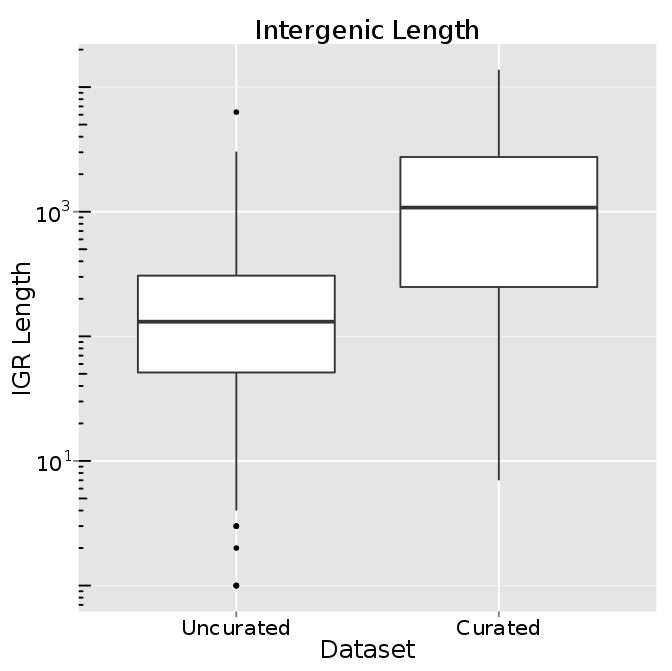
\includegraphics[width=\linewidth,height=3in]{images/Assembly/Curation/PairvsCuration_igrlength.png}
\subcaption{Intragenic Region Lengths}\label{fig:5.21b}}
\end{center}
\end{minipage}%
\end{center}
\caption{UTR and IGR Lengths}
The UTR (\subref{fig:5.21a}) and IGR (\subref{fig:5.21b}) length distributions were considerably improved by the curation method. 
\end{figure}

The transcript length distributions agreed with prokaryotic averages (\ref{fig:5.20a}). Considerable improvements were made to the transcript boundaries from the curation process detailed above. Specifically, the distribution of untranslated region lengths also closely matches \textit{E. coli} averages\cite{87} (\ref{fig:5.21a}). In contrast to the decreased transcript and UTR lengths, intergenic region lengths have increased upon curation (\ref{fig:5.21b}). The curated transcripts are more evenly spaced along the pSol1 megaplasmid than those from the uncurated assembly. Additionally, both the standard and novel transcripts have higher average per-base depth after curation, comparable to the coverage of the reference ORFs (\ref{fig:5.22}). These data show considerable agreement with \textit{E. coli} averages and improvement over the uncurated assembly results. These final transcript coordinates offer pleasing statistics in addition to the precision demonstrated in the previous section.



\begin{figure}
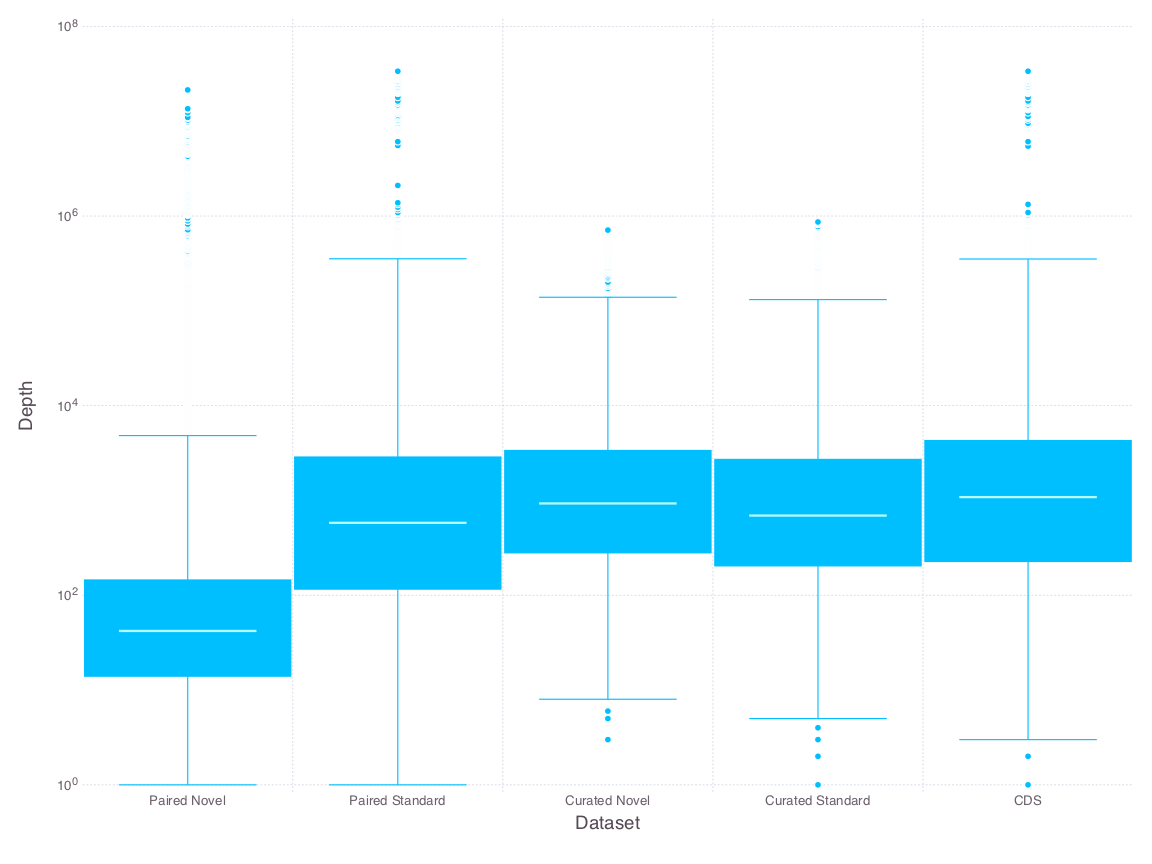
\includegraphics[width=\textwidth]{images/Assembly/Curation/CurvsUncur_boxplot.png}
\caption{Cumulative Depth Distribution}\label{fig:5.22}
\end{figure}


